\documentclass[11pt]{article}

\usepackage{physics}
\usepackage{amsfonts,amsmath,amssymb,amsthm}
\usepackage{enumerate}
\usepackage{titlesec}
\usepackage{fancyhdr}
\usepackage{multicol}

\headheight 13.6pt
\setlength{\headsep}{10pt}
\textwidth 15cm
\textheight 24.3cm
\evensidemargin 6mm
\oddsidemargin 6mm
\topmargin -1.1cm
\setlength{\parskip}{1.5ex}
\parindent=0pt

\author{James Ah Yong}

\pagestyle{fancy}
\fancyhf{}
\fancyfoot[c]{\thepage}
\makeatletter
\lhead{\@title}
\rhead{\@author}

\fancypagestyle{firstpage}{
  \fancyhf{}
  \rhead{\@author}
  \fancyfoot[c]{\thepage}
}

% Sets
\newcommand{\N}{\mathbb{N}}
\newcommand{\Z}{\mathbb{Z}}
\newcommand{\Q}{\mathbb{Q}}
\newcommand{\R}{\mathbb{R}}
\newcommand{\C}{\mathbb{C}}
\newcommand{\U}{\mathcal{U}}
\newcommand{\sym}{\mathbin{\triangle}}

% Functions
\DeclareMathOperator{\sgn}{sgn}
\DeclareMathOperator{\im}{im}

% Operators
\newcommand{\Rarr}{\Rightarrow}
\newcommand{\Larr}{\Leftarrow}
\usepackage{mathtools} % for \DeclarePairedDelimiter macro
\DeclarePairedDelimiter\ceil{\lceil}{\rceil}
\DeclarePairedDelimiter\floor{\lfloor}{\rfloor}

% Macros
% properly typeset ε-δ (epsilon en dash delta)
\newcommand{\epsdel}[1][\delta]{\ensuremath{\epsilon\mathit{\textnormal{--}}#1}}
\newcommand{\by}[1]{& \text{by #1}}
\newcommand{\IH}{\by{inductive hypothesis}}
% multiple choice (remove spacing between items)
\newenvironment{choices}
{\begin{enumerate}[(a)]
    \setlength{\parskip}{0ex}
    }{
  \end{enumerate}}

% Typesetting
\usepackage{array}   % for \newcolumntype macro
\newcolumntype{C}{>{$}c<{$}} % math version of "C" column type
\newcommand{\dlim}[2]{\displaystyle\lim_{#1\to#2}} % totally not \dfrac ripoff
\newcommand{\dilim}[1]{\dlim{#1}{\infty}} % infinite limits
\newcommand{\ilim}[1]{\lim_{#1\to\infty}}
\usepackage{cancel}

% Auto-number questions
\newcommand{\QType}{Q}
\renewcommand{\theparagraph}{\QType\ifnum\value{paragraph}<10 0\fi\arabic{paragraph}}
\setcounter{secnumdepth}{6}
\newcommand{\question}{\par\refstepcounter{paragraph}\textbf{\theparagraph}.\space}

% Question sections
\titleformat{\section}{\normalsize\bfseries}{\thesection}{1em}{}
\newcommand{\qsection}[2]{%
  \renewcommand{\QType}{#2}
  \section*{#1}
  \refstepcounter{section}
}


\title{MATH 135 Fall 2020: Extra Practice 10}

\begin{document}
\thispagestyle{firstpage}

\textbf{\@title}

\qsection{Warm-Up Exercises}{WE}

\question Express $\dfrac{2-i}{3+4i}$ in standard form.
\begin{proof}[Solution]
  Multiply numerator and denominator by the conjugate of the denominator:
  \[ \frac{2-i}{3+4i} = \frac{(2-i)(3-4i)}{9+16} = \frac{2-11i}{25} = \frac{2}{25}-\frac{11}{25}i \qedhere \]
\end{proof}


\question Write $x=\dfrac{9+i}{5-4i}$ in polar form, $r(\cos\theta+i\sin\theta)$, with $0\leq\theta<2\pi$.
\begin{proof}[Solution]
  We express first in standard form by multiplying through the conjugate:
  \[ \frac{9+i}{5-4i} = \frac{(9+i)(5+4i)}{41} = \frac{41+41i}{41} = 1+i \]
  We can geometrically interpret this as $\sqrt2\cis\frac\pi4$.
\end{proof}


\question Write $(\sqrt{3}+i)^4$ in standard form.
\begin{proof}[Solution]
  We first place the quantity within the brackets in polar form.
  By inspection, this is $2\cis\frac\pi6$.
  Now, applying DMT, we have $(2\cis\frac\pi6)^4 = 2^4\cis^4\frac\pi6 = 16\cis\frac{2\pi}{3}$.

  Expressing in standard form,
  $16(\cos\frac{2\pi}{3} + i\sin\frac{2\pi}{3}) = 16(-\frac12+i\frac{\sqrt3}{2}) = -8 + 8\sqrt3 i$
\end{proof}


\question Find all $z\in\C$ such that $z^5=1$ and plot the solutions in the complex plane.
(You may state values in polar form.)
\begin{proof}[Solution]
  Note that $1 = 1\cis0$.
  Applying the CRNT, we have that the five roots are given by
  $\sqrt[5]{1}\cis\left(\frac{2k\pi}{n}\right)$ for $k=0,1,2,3,4$.
  These values are $\{ 1, \cis\frac\pi5, \cis\frac{4\pi}{5}, \cis\frac{6\pi}{5}, \cis\frac{8\pi}{5} \}$.
  I am too lazy to learn \verb|tikz| to draw the diagram.
\end{proof}


\question Find all $z\in\C$ such that $z^2=\dfrac{1+i}{1-i}$.
\begin{proof}[Solution]
  Simplifying the fraction on the right-hand side, $\frac{(1+i)(1+i)}{2}=\frac{1+2i-1}{2}=i$.
  On the complex plane, $i=1\cis\frac\pi2$.
  Then, by CRNT, the solutions are $\cis\frac\pi4$ and $\cis\frac{5\pi}{4}$.
  Evaluating to get standard form, we have $z = \pm(\frac{\sqrt{2}}{2}+\frac{\sqrt{2}}{2}i)$.
\end{proof}


\qsection{Recommended Problems}{RP}

\question Express the following complex numbers in standard form.
\begin{enumerate}[(a)]
  \item $\dfrac{(\sqrt2-i)^2}{(\sqrt2+i)(1-\sqrt2i)}$
        \begin{proof}[Solution]
          Multiply through conjugates of the denominator:
          \begin{align*}
            \frac{(\sqrt2-i)^2}{(\sqrt2+i)(1-\sqrt2i)}
             & = \frac{(1-2\sqrt{2}i)(\sqrt{2}-i)(1+\sqrt{2}i)}{(3)(3)} \\
             & = -\frac{(5-\sqrt2i)(\sqrt2-i)}{9}                       \\
             & = -\frac{4\sqrt2-7i}{9}                                  \\
             & = -\frac{4\sqrt2}{9}+\frac{7}{9}i \qedhere
          \end{align*}
        \end{proof}
  \item $(\sqrt5-i\sqrt3)^4$
        \begin{proof}[Solution]
          Let $z=\sqrt5-i\sqrt3$.
          We have $z^2 = 5 - 2\sqrt{15} i - 3 = 2 - 2\sqrt{15} i$.
          Finally, $z^4 = (z^2)^2 = 4 - 8\sqrt{15} i - 60 = -56 - 8\sqrt{15}i$.
        \end{proof}
\end{enumerate}

\question Prove all of the Properties of Complex Arithmetic that were not proved in the notes or in class.
\begin{proof}
  Let $u=a+bi$, $v=c+di$, and $z=f+gi$ be complex numbers.
  We must show the Properties of Complex Arithmetic, i.e., that
  \begin{enumerate}
    \item Complex addition is associative.

          First, $u+v = (a+c) + (b+d)i$ and $(u+v)+z = ((a+c)+f) + ((b+d)+g)i$.
          Then, $v+z = (c+f) + (d+g)i$, so $u+(v+z) = (a+(c+f)) + (b+(d+g))i$.
          The result follows by the associativity of real addition.

    \item Complex addition is commutative.

          We have $u+v = (a+c) + (b+d)i = (c+a) + (d+b)i = v+u$ by the commutativity of real addition.

    \item The complex additive identity is $0=0+0i$. (Example 3, p. 159)

    \item A complex additive inverse $-z$ exists. (Example 3, p. 159)

    \item Complex multiplication is associative.

          By definition, $uv = (ac-bd)+(ad+bc)i$, so we have
          \[ (uv)w = ((ac-bd)f - (ad+bc)g) + ((ac-bd)g + (ad+bc)f)i \]
          We also have $vw = (cf-dg) + (cg+df)i$ and by extension
          \begin{align*}
            u(vw) & = (a(cf-dg) - b(cg+df)) + (a(cg+df) + b(cf-dg))i      \\
                  & = (acf - adg - bcg - bdf) +  (acg + adf + bcf - bdg)i \\
                  & = (acf - bdf - adg - bcg) +  (acg - bdg + adf + bcf)i \\
                  & = ((ac-bd)f - (ad+bc)g) + ((ac-bd)g + (ad+bc)f)i      \\
                  & = (uv)w
          \end{align*}
          as desired.

    \item Complex multiplication is commutative.

          Again, $uv = (ac-bd)+(ad+bc)i$ and $vu = (ca-db)+(cb+da)i$.
          The result follows from the commutativity of real multiplication and addition.

    \item The complex multiplicative identity is $1=1+0i$. (Example 3, p. 159)

    \item A complex multiplicative inverse $z^{-1}$ exists iff $z \neq 0$.
          (Proposition 1, p. 159)

    \item Complex multiplication distributes over addition.

          We have $u+v = (a+c) + (b+d)i$. Then,
          \[ z(u+v) = (f(a+c) - g(b+d)) + (f(b+d) + g(a+c))i \]
          Now, $zu = (fa - gb) + (fb + ga)i$ and $zv = (fc - gd) + (fd + gc)i$, so by definition,
          \begin{align*}
            zu + zv & = ((fa - gb) + (fc - gd)) + ((fb + ga) + (fd + gc))i \\
                    & = (fa + fc - gb - gd) + (fb + fd + ga + gc)i         \\
                    & = (f(a+c) - g(b+d)) + (f(b+d) + g(a+c))i             \\
                    & = z(u+v)
          \end{align*}
          completing the proof. \qedhere
  \end{enumerate}
\end{proof}


\question Let $n \in \N$. Prove that if $n \equiv 1 \pmod 4$, then $i^n = i$.
\begin{proof}
  Let $n$ be a natural number congruent to 1 modulo 4.
  Then, we may write $n = 4k+1$ for some integer $k$.
  Notice that $i^4 = (i^2)^2 = (-1)^2 = 1$.

  Therefore, $i^{4k+1} = (i^4)^k i^1 = (1)^k i = i$, as desired.
\end{proof}


\question Find all $z \in \C$ which satisfy
\begin{enumerate}[(a)]
  \item $z^2+2z+1=0$
        \begin{proof}[Solution]
          Factor: $z^2 + 2z + 1 = (z+1)^2$ so $z = -1 + 0i$ (by~\ref{q:fac})
        \end{proof}
  \item $z^2+2\bar{z}+1=0$
        \begin{proof}[Solution]
          Let $z=a+bi$ so $\bar{z}=a-bi$ for two real numbers $a$ and $b$. Then,
          \begin{align*}
            0 & = z^2+2\bar{z}+1           \\
            0 & = (a+bi)^2+2(a-bi)+1       \\
            0 & = (a^2+2a-b^2+1)+(2ab-2b)i
          \end{align*}
          which is true if and only if both $a^2+2a-b^2+1=0$ and $2ab-2b=0$.

          The second equation implies $2ab=2b$ so $a=1$ or $b=0$.

          If $a=1$ then $a^2+2a-b^2+1 = 4-b^2 = 0$, so $b=\pm 2$.

          If $b=0$, then $a^2+2a+1 = (a+1)^2 = 0$, so $a = -1$.

          Therefore, the solutions are $-1+0i$, $1+2i$, and $1-2i$.
        \end{proof}
  \item $z^2 = \dfrac{1+i}{1-i}$
        \begin{proof}[Solution]
          Simplify: $z^2 = \frac{(1+i)^2}{2} = \frac{2i}2 = i$.
          The square roots of $i$ are $\pm (\frac{\sqrt{2}}{2} + \frac{\sqrt{2}}{2}i)$.
        \end{proof}
\end{enumerate}


\question \begin{enumerate}[(a)]
  \item Find all $w\in\C$ satisfying $w^2 = -15 + 8i$.
        \begin{proof}[Solution]
          We rewrite $w=a+bi$ for some reals $a$ and $b$.
          Then, $(a+bi)^2 = (a^2 - b^2) + (2ab)i = -15 + 8i$.
          Equating real and complex parts, $a^2 - b^2 = -15$ and $2ab = 8$.

          Now, $|w^2| = |ww| = |w| |w| = |w|^2$ by PM4.
          Then, $a^2+b^2 = \sqrt{(-15)^2 + (8)^2} = 17$.
          Solving the system in $a^2$ and $b^2$, $a^2 = 1$ and $b^2 = 16$.

          Therefore, $a = \pm 1$ and $b = \pm 4$.
          To satisfy $2ab=8$, we must have $z = \pm(1 + 4i)$.
        \end{proof}
  \item Find all $z\in\C$ satisfying $z^2-(3+2i)z+5+i=0$.
        \begin{proof}[Solution]
          We apply the quadratic formula.
          The discriminant is a solution to $w^2 = (3+2i)^2 - 4(1)(5+i) = (5+12i) - (20+4i) = -15+8i$.
          From above, a solution is $w=1+4i$.
          Therefore, the solutions are $z = \frac{(3+2i) \pm (1+4i)}{2(1)}$.

          The first is $z = \frac{(3+2i) + (1+4i)}{2} = 2+3i$
          and the second is $z = \frac{(3+2i) - (1+4i)}{2} = 1-i$.
        \end{proof}
\end{enumerate}


\question\label{q:fac} Let $z, w \in \C$. Prove that if $zw = 0$ then $z = 0$ or $w = 0$.
\begin{proof}
  Let $z$ and $w$ be complex numbers such that $zw = 0$.
  Suppose for a contradiction that both $z$ and $w$ are non-zero.
  Then, by PM1, $|z| \neq 0$ and $|w| \neq 0$.
  However, by PM4, $|zw| = |z| |w| \neq 0$, which is a contradiction, since $zw = 0$.

  Therefore, $z$ or $w$ is zero.
\end{proof}


\question Let $a,b,c \in \C$. Prove: if $|a|=|b|=|c|=1$,
then $\overline{a+b+c}=\frac1a+\frac1b+\frac1c$.
\begin{proof}
  First, consider some arbitrary complex number $z=a+bi$ with modulus 1.
  By definition, $a^2 + b^2 = 1^2 = 1$.
  Then, $z^{-1} = \frac{1}{a+bi} = \frac{a-bi}{(a+bi)(a-bi)} = \frac{a-bi}{1} = a-bi = \bar{z}$

  Let $a$, $b$, and $c$ be complex numbers with modulus 1.
  From above, $a^{-1}=\bar{a}$, $b^{-1}=\bar{b}$, and $c^{-1}=\bar{c}$.
  The conclusion immediately follows from PCJ2:
  \begin{align*}
    \overline{a+b+c} & = \bar{a} + \bar{b} + \bar{c}          \\
                     & = \frac1a+\frac1b+\frac{1}{c} \qedhere
  \end{align*}
\end{proof}


\question Find all $z\in\C$ satisfying $z^2=|z|^2$.
\begin{proof}
  Let $z$ be a complex number.
  Recall that $|z|^2 = \bar{z}z$ by PM3.
  Then, we have $z^2 = \bar{z}z$ so $z = \bar{z}$, that is, $z - \bar{z} = 0$.
  By PCJ3, this is true if $2\Im(z)i = 0$, which means that $z$ is purely real.
  Therefore, $z$ is any purely real number.
\end{proof}


\question Find all $z\in\C$ satisfying $|z+1|^2 \leq 3$ and shade the corresponding region in the complex plane.
\begin{proof}[Solution]
  We write $z = a+bi$, so $|z+1|^2 = |(a+1)+bi|^2 = (\sqrt{(a+1)^2+b^2})^2 = (a+1)^2 + b^2$.
  Then, we are shading the inside of the circle defined by $(a+1)^2 + b^2 = 3$.
  \begin{center}
    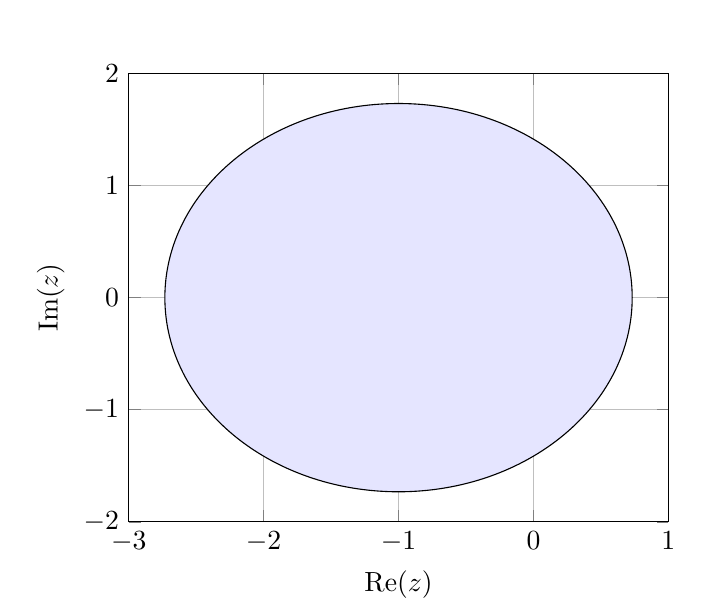
\begin{tikzpicture}
      \begin{axis}[
          xlabel=$\Re(z)$, ylabel=$\Im(z)$,
          xmin=-3, xmax=1, ymin=-2, ymax=2, grid=both]
        \draw[fill=blue!10] (axis cs:-1,0) circle[radius=sqrt(3)];
      \end{axis}
    \end{tikzpicture}
  \end{center}
  This is the circle centered at $(-1,0)$ with radius $\sqrt3$.
\end{proof}


\question Let $z,w\in\C$ such that $\overline{z} w \neq 1$.
Prove that if $|z|=1$ or $|w|=1$, then $\abs{\dfrac{z-w}{1 - \overline{z} w}}=1$.
\begin{prf}[by sooshi]
  Let $z$ and $w$ be complex numbers such that $\overline{z} w \neq 1$.
  Suppose that $|z| = 1$ or $|w| = 1$.
  If $z = w$ and $|z| = |w| = 1$, then $\overline{z}w = \overline{z}z = |z|^2 = 1$.
  Therefore, $z \neq w$.

  Now, consider the case when $|z| = 1$. Then,
  \begin{equation*}
    \abs{\frac{z-w}{1 - \overline{z} w}}
      = \frac{|z-w|}{|1 - \overline{z} w|}       
      = \frac{|z||z-w|}{|z||1 - \overline{z} w|} 
      = \frac{(1)|z-w|}{|z - z\overline{z}w|}       
      = \frac{|z-w|}{|z-w|}
      = 1
  \end{equation*}
  Likewise, if $|w| = 1$, then
  \begin{equation*}
    \abs{\frac{z-w}{1 - \overline{z} w}}
     = \frac{|z-w|}{|1 - \overline{z} w|}            
     = \frac{|z-w|}{|w\overline{w} - \overline{z} w|}
     = \frac{|z-w|}{|w||\overline{w} - \overline{z}|}
     = \frac{|z-w|}{|w-z|}                           
     = 1
  \end{equation*}
  since $|w-z| = \abs{-(z-w)} = \abs{-1}|z-w| = |z-w|$, completing the proof.
\end{prf}


\question Show that for all complex numbers $z$, $|\Re(z)|+|\Im(z)|\leq\sqrt{2}|z|$.
\begin{proof}
  Let $z = r\cis \theta$ be a complex number.
  Then, $|z| = r$, $\Re(z) = r\cos\theta$ and $\Im(z) = r\sin\theta$.
  Due to the symmetry of sine and cosine, instead of taking absolute values,
  we restrict without loss of generality to the first quadrant $0 \leq \theta \leq \frac\pi2$. Now,
  \begin{align*}
    \Re(z) + \Im(z) & = r(\cos\theta + \sin\theta)                                                          \\
                    & = r\sqrt{2}\frac{\sqrt{2}}{2}(\cos\theta + \sin\theta)                                \\
                    & = r\sqrt{2}\left( \frac{\sqrt{2}}{2}\cos\theta + \frac{\sqrt{2}}{2}\sin\theta \right) \\
                    & = r\sqrt{2}\left( \sin\frac\pi4\cos\theta + \cos\frac\pi4\sin\theta \right)           \\
                    & = r\sqrt{2}\sin\left(\frac\pi4 + x\right)                                             \\
                    & \leq r\sqrt{2}(1)                                                                     \\
                    & = \sqrt{2}|z|
  \end{align*}
  completing the proof.
\end{proof}


\question Use \emph{De Moivre's Theorem} (DMT) to prove that
$\sin 4\theta = 4\sin\theta\cos^3\theta - 4\sin^3\theta\cos\theta$ for all $\theta\in\R$.
\begin{proof}
  Let $\theta \in \R$ and note that by DMT, we have
  \[ (\cos\theta + i\sin\theta)^4 = \cos 4\theta + i\sin 4\theta \]
  so we may say that $\sin 4\theta = \Im((\cos\theta + i\sin\theta)^4)$.
  Expanding this quantity by hand,
  \begin{align*}
    (\cos\theta + i\sin\theta)^4
     & = (\cos^2 \theta + 2i\cos\theta\sin\theta - \sin^2\theta)^2                                                        \\
     & = \cos^4\theta + \sin^4\theta - 2\cos^2\theta\sin^2\theta + 4i\cos^3\theta\sin\theta - 4i\sin^3\theta\cos\theta    \\
     & = (\cos^4\theta - 2\cos^2\theta\sin^2\theta + \sin^4\theta) + (4\cos^3\theta\sin\theta - 4\sin^3\theta\cos\theta)i
  \end{align*}
  and we have that
  \[ \sin 4\theta = \Im((\cos\theta + i\sin\theta)^4) = 4\cos^3\theta\sin\theta - 4\sin^3\theta\cos\theta \]
  as desired.
\end{proof}


\question Let $n\in\N$ and $a,b\in\R$. Show that $z=(a+bi)^n+(a-bi)^n$ is real.
\begin{proof}
  Let $n$ be a natural number and $u=a+bi$ be a complex number. Then, $\overline{u}=a-bi$.
  It inductively follows from PCJ4 and the associativity of multiplication
  that $(\overline{u})^n = \overline{u^n}$.

  Now, the fact that $z = u^n + \overline{u^n}$ is real follows immediately from PCJ3.
\end{proof}


\question An \emph{$n$-th root of unity} is any complex solution to $z^n=1$.
Prove that if $w$ is an $n$-th root of unity, $\frac1w$ is also an $n$-th root of unity.
\begin{proof}
  Let $n$ be a natural number and $w$ be an $n$-th root of unity, so $w^n = 1$.
  Knowing that $1=\cis0$, the CNRT states that $w = \cis(\frac{2k\pi}{n})$ for some $0 \leq k < n$.

  By PM\C, notice that $w\cis(-\frac{2k\pi}{n}) = \cis(\frac{2k\pi}{n}-\frac{2k\pi}{n}) = \cis 0 = 1$,
  so $\cis(-\frac{2k\pi}{n})$ is the multiplicative inverse $w^{-1}$ of $w$.
  Now, since $\cis$ is $2\pi$-periodic, we have
  \[
    \cis\left(-\frac{2k\pi}{n}\right) = \cis\left(2\pi-\frac{2k\pi}{n}\right)
    = \cis\left(\frac{2n\pi-2k\pi}{n}\right) = \cis\left(\frac{2(n-k)\pi}{n}\right)
  \]
  but since $0 \leq k < n$, we also have that $0 \leq n-k < n$.
  Therefore, by the CNRT, $w^{-1}$ is an $n$-th root of unity.
\end{proof}


\question A complex number $z$ is called a \emph{primitive} $n$-th root of unity
if $z^n=1$ and $z^k \neq 1$ for all $1 \leq k \leq n-1$.
\begin{enumerate}[(a)]
  \item For each $n=1,3,5,6$ list all the primitive $n$-th roots of unity.
        \begin{proof}[Solution]
          Recall that $1^x=1$ for any real $x$.
          Applying the CNRT, there are $n$ $n$-th roots of unity, of the form
          \[ z = \cis\left(\frac{2\pi k}{n}\right) \]
          for some integer $0 \leq k < n$.
          Note that 1 is always an $n$-th root of unity but only a primitive first root of unity.
          Therefore, we can ignore the case $k=0$.

          The only primitive 1st root of unity is 1.

          The primitive 3rd roots of unity are
          $\cis \frac{2\pi}{3} = \frac{\sqrt 3}{2} - \frac{1}{2}i$ and
          $\cis \frac{4\pi}{3} = \frac{\sqrt 3}{2} + \frac{1}{2}i$.

          For this, we remain in polar form as calculating sines and cosines of fractions over 5 is \emph{pain}.
          The primitive 5th roots of unity are $\cis 0 = 1$, $\cis \frac{2\pi}{5}$, $\cis \frac{4\pi}{5}$,
          $\cis \frac{6\pi}{5}$, and $\cis \frac{8\pi}{5}$.

          The 6th roots of unity are $\cis \frac{2\pi k}{6} = \cis \frac{\pi k}{3}$.
          However, when $k=2$, $k=3$, and $k=4$, these are also 2nd/3rd roots of unity.
          Thus, the primitive roots of unity are
          $\cis \frac{\pi}{3} = \frac{1}{2} + \frac{\sqrt{3}}{2}i$ and
          $\cis \frac{5\pi}{3} = \frac{1}{2} - \frac{\sqrt{3}}{2}i$.
        \end{proof}
  \item Let $z$ be a primitive $n$-th root of unity. Prove the following statements:
        \begin{enumerate}[i.]
          \item For any $j\in\Z$, $z^j=1$ if and only if $n \mid j$.
                \begin{proof}
                  Let $n$ be a natural number, $j$ be an integer,
                  and $z$ be a primitive $n$-th root of unity so $z^n=1$.
                  Proceed by mutual implication.

                  ($\Rarr$) Suppose $z^j = 1$.
                  By the Division Algorithm, $j = qn + r$ for integers $q$ and $0 \leq r < n$.
                  Then, $1 = z^j = z^{qn+r} = z^{qn}z^r = (z^n)^q z^r = 1^q z^r = z^r$.

                  If $r=0$, then $j = qn$ and $j \mid n$.
                  Otherwise, we have $1 \leq r \leq n-1$ and $z^r = 1$, which is a contradiction
                  to the fact that $z$ is a primitive $n$-th root of unity.

                  Therefore, $r = 0$ and $j \mid n$.

                  ($\Larr$) If $n \mid j$ and $j = nk$ for an integer $k$,
                  then $z^j = z^{nk} = (z^n)^k = 1^k = 1$.
                \end{proof}
          \item For any $m\in\Z$, if $\gcd(m,n)=1$, then $z^m$ is a primitive $n$-th root of unity.
                \begin{prf}[new and improved by sooshi]
                  Let $z$ be a primitive $n$-th root of unity and $m$ an integer coprime to $n$.
                  
                  Suppose for a contradiction that $z^m$ is a $k$-th root of unity for some $1 \leq k < n$.
                  Then, $(z^m)^k = z^{mk} = 1$.
                  From above, this implies that $n \mid mk$ and by CAD, $n \mid k$.
                  However, BBD gives that $n \leq k$, which is a contradiction.

                  Therefore, $z^m$ is a primitive $n$-th root of unity.
                \end{prf}
        \end{enumerate}
\end{enumerate}


\question Let $u$ and $v$ be fixed complex numbers.
Let $\omega$ be a non-real cube root of unity.
For each $k\in\Z$, define $y_k\in\C$ by the formula \[ y_k = \omega^k u + \omega^{-k}v \]
\begin{enumerate}[(a)]
  \item Compute $y_1$, $y_2$, and $y_3$ in terms of $u$, $v$, and $\omega$.
        \begin{proof}[Solution]
          From RP15(a), the only real cube root of unity is 1, so $\omega \neq 1$.
          In fact, $\omega = \cis \frac{n\pi}{3}$ for either $n=2$ or $n=4$.

          If $n=2$, then $\omega^{-1} = \cis \frac{-2\pi}{3} = \cis\frac{4\pi}{3}$.
          If $n=4$, then $\omega^{-1} = \cis \frac{-4\pi}{3} = \cis\frac{2\pi}{3}$.

          However, using the standard form from RP15(a), $\cis\frac{2\pi}{3} = \overline{\cis\frac{4\pi}{3}}$.
          Therefore, $\omega^{-1} = \overline{\omega}$.

          Now, $y_1 = \omega u + \overline{\omega} v$,
          $y_2 = \omega^2 u + \overline{\omega}^2 v$, and
          $y_3 = \omega^3 u + \overline{\omega}^3 v = u + v$.
        \end{proof}
  \item Show that $y_k = y_{k+3}$ for any $k\in\Z$.
        \begin{proof}
          Let $k$ be an integer.
          Then, knowing that both $\omega$ and $\overline{\omega}$ are cube roots of unity,
          \begin{align*}
            y_{k+3} & = \omega^{k+3} u + \overline{\omega}^{k+3} v                      \\
                    & = \omega^k \omega^3 u + \overline{\omega}^k \overline{\omega}^3 v \\
                    & = \omega^k u + \overline{\omega}^k v                              \\
                    & = y_k
          \end{align*}
          completing the proof.
        \end{proof}
  \item Show that for any $k\in\Z$, \[ y_k-y_{k+1} = \omega^k(1-\omega)(u-\omega^{k-1}v) \]
        \begin{proof}
          Let $k$ be an integer. Expand the right-hand side:
          \begin{align*}
            \omega^k(1 - \omega)(u - \omega^{k-1}v)
             & = (\omega^k-\omega^{k+1})(u-\omega^{k-1}v)                         \\
             & = \omega^k u - \omega^{2k+1}v - \omega^{k+1}u + \omega^{2k+2}v     \\
             & = (\omega^k u + \omega^{2k+2}v) - (\omega^{k+1}u + \omega^{2k+1}v)
          \end{align*}
          To simplify, we show that $\omega^{2k+2} = \omega^{-k}$.
          Equivalently, $\omega^{2k+2}\omega^k = \omega^{3k+2} = 1$.
          Let $j = k+1$. Then,
          \[ \omega^{3k+2} = \omega^{3(j-1)+2} = \omega^{3j-1} = (\omega^3)^j \omega^{-1} = 1^j \omega^{-1} = \omega^{-1} \]
          as desired.
          Now, we have $\omega^{2k+2} = \omega^{-k}$ and $\omega^{2k+1} = \omega^{-(k+1)}$ so
          \begin{align*}
            \omega^k(1 - \omega)(u - \omega^{k-1}v)
             & = (\omega^k u + \omega^{2k+2}v) - (\omega^{k+1}u + \omega^{2k+1}v) \\
             & = (\omega^k u + \omega^{-k}v) - (\omega^{k+1}u + \omega^{-(k+1)}v) \\
             & = y_k - y_{k+1} \qedhere
          \end{align*}
        \end{proof}
\end{enumerate}


\qsection{Challenges}{C}

\question Let $z,w\in\C$.
\begin{enumerate}[(a)]
  \item Prove that $|z+w| \leq |z| + |w|$.
        \begin{proof}
          This is the Triangle Inequality, for which a geometric proof is provided in Chapter 10.3.
          In short, for complex numbers $z = a+bi$ and $w = c+di$,
          we consider a triangle $\triangle OZW$ with points $O(0,0)$, $Z(a,b)$, and $W(c,d)$ in the complex plane.
          Then, $|z| = \ell_{OZ}$, $|w| = \ell_{OW}$, and $|z+w| = \ell_{ZW}$.
          The length of one side of a triangle cannot exceed the sum of the lengths of the other two sides.

          Equivalently, $\ell_{ZW} \leq \ell_{OZ} + \ell_{OW}$.
        \end{proof}
  \item Prove that $\abs{|z| - |w|} \leq |z-w| \leq |z|+|w|$.
        \begin{proof}
          Let $z$ and $w$ be complex numbers.
          We prove the inequalities separately.

          We apply the Triangle Inequality with $z$ and $-w$.
          Then, $|z + (-w)| \leq |z| + |-w|$ but $|-w| = |-1||w| = |w|$ by PM4,
          so we have $|z-w| \leq |z| + |w|$.

          Now, notice that $|z| = |(z-w) + w| \leq |z-w| + |w|$ so $|z| - |w| \leq |z-w|$.

          Likewise, $|w| = |(w-z) + z| \leq |w-z| + |z|$ so $|z| - |w| \geq -|w-z|$.

          Like the absolute value in \R, we have by PM4 $|w-z| = |-1||z-w| = 1|z-w| = |z-w|$,
          so if we combine the above two inequalities, we have $\abs{|z| - |w|} \leq |z-w|$.

          Equivalently, using the same triangle from above, this follows from the fact that
          any one side of a triangle is longer than the difference of the other two sides.
        \end{proof}
\end{enumerate}

\question Let $a,b,c\in\C$.
Show that if $\dfrac{b-a}{a-c} = \dfrac{a-c}{c-b}$ then $|b-a| = |a-c| = |c-b|$.

\question Let $n \geq 2$ be an integer. Prove that
\[ \sum_{k=0}^{n-1}\cos\left(\frac{2k\pi}{n}\right)=0=\sum_{k=0}^{n-1}\sin\left(\frac{2k\pi}{n}\right) \]
\begin{prf}[with help from Ainsley, Kenson, Mabel]
  Let $n \neq 1$ be a natural number.
  Then, we have that the $n$-th roots of unity are given by
  \[ \cos(\frac{2k\pi}{n}) + i \sin(\frac{2k\pi}{n}) \]
  for $k = 0,1,2,\ldots,n-1$.
  Let $z$ be the sum of the $n$-th roots of unity. Then,
  \[ z = \sum_{k=0}^{n-1}\left(\cos(\frac{2k\pi}{n}) + i\sin(\frac{2k\pi}{n})\right) \]
  The conclusion can equivalently be stated as that $\Re(z) = 0$ and $\Im(z) = 0$.
  The only complex number that satisfies this is $z = 0$.

  Now, let $a = \cos(\frac{2\pi}{n}) + i\sin(\frac{2\pi}{n})$, the root of unity with $k = 1$.
  Then, we have that each root of unity is given by $a^j$ for $j = 1,2,\ldots,n$.
  Since $n \neq 1$, $a = \cis\frac{2\pi}{n} \neq 1$ and $z = 1 + a + a^2 + \cdots + a^{n-1}$.

  Recall that the polynomial $a^n - 1$ for $n \geq 2$ factors as
  $(a-1)(a^{n-1} + a^{n-2} + \cdots + a^2 + a + 1)$.
  It follows that $a^n - 1 = 1-1 = 0$ and $0 = (a-1)z$ so, from above, $a \neq 1$ so $z = 0$.
\end{prf}

\end{document}